\documentclass[../main.tex]{subfiles}
\begin{document}

\subsection{Aufbau}
    Der Versuchsapparat (siehe Abbildung \ref{fig:Versuchsaufbau}) besteht aus drei ineinander verschachtelten Spulen, die an ein Spektrometer angeschlossen sind:
    \begin{itemize}
        \item Die äußerste \textbf{Polarisationsspule} dient dem Erzeugen von Polarisationspulsen, für eine Präperation der Kernspins.
        \item Die mittlere \textbf{Gradientenspule} stellt, wenn nötig, zusätzliche lineare Inhomogenitäten des äußeren B-Felds bereit. Dies wird einerseits dazu genutzt, B-Feld Inhomogenitäten innerhalb der Probe zu kompensieren. Anderseits kann durch einen nicht-verschwindenen Gradienten einen räumliche Auflösung von Messungen erzielt werden.
        \item Die innerste \textbf{$B_1$-Spule} hat zwei Aufgaben: eine Anregung der Probe durch einen $B_1$-Feld-Puls und die Messung der darauffolgenden Antwort, bezeichnet als \textit{H-Signal}.
    \end{itemize}
    Innerhalb der innersten Spule kann die Probe platziert werden. Das externe B-Feld wird durch das Erdmagnetfeld $B_0$ bereitgestellt. Alle Daten werden mithilfe von der \textit{Prospa}-Software von Magritek ausgelesen.\\
    
    Wird durch die $B_1$-Spule eine Präzession der Magnetisierung der Probe erzeugt, so wird nach dem \textit{Faraday'schen Induktionsgesetz} eine sinusförmige Spannung in derselben Spule induziert. Diese bildet mit einem Kondensator $C$ im Spektrometer einen LCR-Schwingkreis; tatsächlich gemessen werden die Spannungsschwingungen dort.

    \begin{figure}[H]
        \centering
        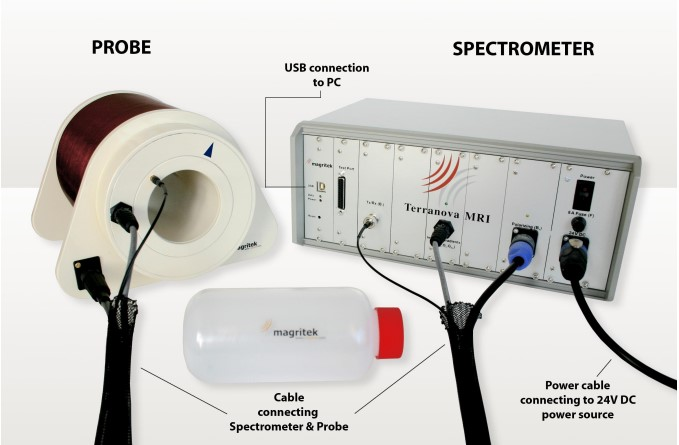
\includegraphics[width=0.7\textwidth]{Bilddateien/Versuchsaufbau.jpg}
        \caption{Spule und Spektrometer des Versuchsapparates \cite[p.10]{doc:EFNMRStudentManual}}
        \label{fig:Versuchsaufbau}
    \end{figure}

\newpage
\subsection{Durchführung}
    Falls nicht explizit anders erwähnt, ist die genutzte Probe Wasser. 

    \paragraph{Bestimmung der Larmor-Frequenz}.
        Zunächst wird in der Prospa-Software ein \textit{Pulse-and-Collect}-Experiment durchgeführt:
        \begin{center}
            Polarisationspuls $\rightarrow$ warte $\rightarrow$ $\pi$-Puls.
        \end{center}
        In Tabelle \ref{tab:DurchfuehrungTeil2Parameter} sind die ursprünglichen Parameter aufgeführt. Die Larmor-Frequenz $f_L$ der H-Atome ergibt sich durch den spektralen Peak des aufgenommen H-Signals.

        \begin{table}[H]
            \centering
            \begin{tabular}{cc|cc}
                 \textbf{Parameter} & \textbf{Wert} & \textbf{Parameter} & \textbf{Wert}  \\\hline\hline
                Polarizing current (\si{\ampere}) & 6 & Number data points & 16384\\\hline
                Polarizing duration (\si{\milli\second}) & 4000 & Aquisition delay (\si{\milli\second}) & 25\\\hline
                $B_1$ frequency (\si{\hertz}) & 2012 & Acquisition time (\si{\second}) & \num{1.5}\\\hline
                Capacitance (\si{\nano\farad}) & \num{10.8} & Repetition time (\si{\second}) & 8\\\hline
                Transmit $B_1$ gain & 2 & Number of scans & 4\\\hline
                Pulse duration (\si{\milli\second}) & \num{1.5} & Display range (\si{\hertz}) & 600\\\hline
                Receive gain & 2 & Average/ Magnitude & Ja
            \end{tabular}
            \caption{\textit{Pulse-and-Collect} Parameter zur Bestimmung der Larmorfrequenz.}
            \label{tab:DurchfuehrungTeil2Parameter}
        \end{table}

    \paragraph{Rauschsignal messen.}
        Als nächstes wird das Hintergrundrauschen mit einem \textit{MonitorNoise}-Experiment vermessen. Es wird kein Puls von der $B_1$-Spule ausgesandt! Die relevanten Parameter sind in Tabelle \ref{DurchfuehrungTeil3Parameter} aufgeführt.  

        \begin{table}[H]
            \centering
            \begin{tabular}{cc|cc}
                 \textbf{Parameter} & \textbf{Wert} & \textbf{Parameter} & \textbf{Wert}  \\\hline\hline
                $B_1$ frequency (\si{\hertz}) & $f_L$ & Number data points & 16384\\\hline
                Capacitance (\si{\nano\farad}) & \num{10.8} & Acquisition time (\si{\second}) & \num{0.5}\\\hline
                Receive gain & 2 & Number of scans & 40\\\hline
                Time amplitude & 50 & Frequency amplitude & 10\\\hline
                Display range (\si{\hertz}) & 5500 & - & -
            \end{tabular}
            \caption{\textit{MonitorNoise} Parameter zur Vermessung des Rauschens der Probe.}
            \label{tab:DurchfuehrungTeil3Parameter}
        \end{table}

    \paragraph{Parameteroptimierung für ein klares H-Signal.}
        Für ein möglichst klares H-Signal ist es von Vorteil, dass:
        \begin{enumerate}
            \item die LCR-Resonanzfrequenz $f_R$ und die Larmorfrequenz $f_L$ zusammenfallen. Um die passende Kapazität $C_L$ auswählen zu können, wird nun der Zusammenhang $f_R(C)$ untersucht. Hierfür ist das \textit{AnalyseCoil}-Experiment geeignet. Als Parameter werden dieselben wie in \ref{tab:DurchfuehrungTeil2Parameter} verwendet, nur die \textit{$B_1$ frequency} wird durch $f_L$ ersetzt.
 
            
            \item die $B_1$-Pulslänge $\tau_A$ eine maximale Amplitude $A$ des H-Signals hervorruft. Das \textit{$B_1$-Duration}-Experiment liefert hierzu den Zusammenhang $A(\tau)$. In Tabelle sind die genutzten Parameter bereitgestellt.\\

            \begin{table}[H]
                \centering
                \begin{tabular}{cc|cc}
                    \textbf{Parameter} & \textbf{Wert} & \textbf{Parameter} & \textbf{Wert}  \\\hline\hline
                    Polarizing current (\si{\ampere}) & 6 & Number data points & 16384\\\hline
                    Polarizing duration (\si{\milli\second}) & 4000 & Aquisition delay (\si{\milli\second}) & 25\\\hline
                    $B_1$ frequency (\si{\hertz}) & $f_L$ & Acquisition time (\si{\second}) & \num{1.5}\\\hline
                    Capacitance (\si{\nano\farad}) & $C_L$ & Repetition time (\si{\second}) & 8\\\hline
                    Transmit $B_1$ gain & 2 & Number of scans & 4\\\hline
                    Minimum $B_1$ duration (\si{\milli\second}) & \num{0.25} & Display range (\si{\hertz}) & 300\\\hline
                    Number $B_1$ steps & 26 & Integration range (\si{\hertz}) & 50\\\hline
                    $B_1$ step size (\si{\milli\second}) & \num{0.25} & Receive gain & 2\\\hline
                    Filter & Ja & Average & Nein
                \end{tabular}
                \caption{\textit{$B_1$-Duration} Parameter zur Bestimmung der optimalen Anregungspulslänge.}
                \label{tab:DurchfuehrungTeil3ParameterB1Duration}
            \end{table}


            \textbf{Achtung}: Wegen einer technischen Einschränkung des Apparats wird nicht das $\tau_M$ mit maximalen $A(\tau_M)$ als optimalen Parameter gewählt - sondern das Vielfache der halben Periodendauer zu $f_L$, welches diesem $\tau_M$ am Nächsten kommt. Auch die \textit{Minimum $B_1$ duration} und \textit{$B_1$ step size} müssen Vielfahce der halben Periodendauer seien. 
            
            \item das äußere B-Feld ($B_0$ plus zusätzliche Störungen) innerhalb der Probe homogen ist. Dazu findet das \textit{AutoShim}-Experiment automatisch optimale Parameter, sodass die Gradientenspule ungewollte Inhomogenitäten kompensiert.
        \end{enumerate}

        Nach der Kalibrierung wird nochmals ein H-Signal im \textit{Pulse-and-Collect}-Experiment aufgenommen. Die gefunden Parameter werden auch im folgenden Versuchsverlauf genutzt.
    
    \paragraph{Untersuchung der longitudinalen Spin-Gitter-Relaxation.}
        Im Folgenden wird auch die Präperation der Probe durch den Polarisationspuls untersucht. Genauer gesagt, wird gemessen, wie die Wechselwirkung der Kernspins mit der lokalen Umgebung sich in der Abhängigkeit der H-Signalstärke $S$ von der Polarisationspulsdauer $\tau_P$ manifestiert. Durch Iteration vieler \textit{Pulse-and-Collect}-Experiment kann $S(\tau_P)$ im \textit{$T_1$-$B_p$}-Experiment erhalten werden. Tabelle \ref{tab:DurchfuehrungTeil8Parameter} listet die verwendeten Parameter auf.

         \begin{table}[H]
            \centering
            \begin{tabular}{cc|cc}
                 \textbf{Parameter} & \textbf{Wert} & \textbf{Parameter} & \textbf{Wert}  \\\hline\hline
                Polarising current (\si{\ampere}) & 6 & Transmit ($B_1$) gain & \num{2.0}\\\hline
                Minimum polarizing time (\si{\milli\second}) & 250 & 90 pulse duration (\si{\milli\second}) & $\tau_A$\\\hline 
                Polarizing step size (\si{\milli\second}) & 400 & Receive Gain & 2\\\hline
                Number of steps & 20 & 90-acquisition delay (\si{\milli\second}) & 25\\\hline 
                $B_1$ frequency (\si{\hertz}) & $f_L$ & Number of data points & 16384\\\hline
                Capacitance (\si{\nano\farad}) & $C_L$ & Acquisition time (\si{\second}) & \num{1.5}\\\hline
                Repetition time (\si{\second}) & \num{13.1} & Number of scans & 4\\\hline
                Integration width (\si{\hertz}) & 50 & Display range (\si{\hertz}) & 200\\\hline
                Average/ Magnitude & Ja & Filter & Nein
            \end{tabular}
            \caption{\textit{$T_1$-$B_p$} Parameter zur Bestimmung der Abhängigkeit der H-Signalstärke von der Polarisationspulsdauer. Die Signalamplitde wird durch Integration des spektralen Peaks erhalten, das Integrationsgebiet ist durch \textit{Integration width} gegeben.}
            \label{tab:DurchfuehrungTeil8Parameter}
        \end{table}

    \paragraph{Erzeugung von Spin-Echos.}
        Ein weiterer Störfaktor des H-Signals ist, dass die Kernspins durch Spin-Spin-Wechselwirkung oder lokale Inhomogenitäten des $B$-Feld ihre Kohärenz zueinander verlieren. Durch aufeinanderfolgende Pulse kann letzterer Effekt kompensiert werden.  Der Ablauf des \textit{Spin-Echo}-Experiments (mit Shims) ist:
        \begin{center}
            Polpuls. $\longrightarrow$ warte $\longrightarrow$ $\pi/2$-Puls $\longrightarrow$ warte $\tau_E$ $\longrightarrow$ $\pi$-Puls.
        \end{center}

        Um zu untersuchen, inwiefern diese Kompensation interner (Spin-Echo) und externer (Shimming) Inhomogenitäten des $B$-Felds effektiv sind, wird das Experiment durchgeführt für:
        \begin{itemize}
            \item optimale Shimming Parameter.
            \item einem zu großen/ kleinen $x$-Shimming Parameter.
        \end{itemize}

        Die verwendenten Schimming-Parameter sind in Tabelle \ref{tab:DurchfuehrungTeil9ParameterShimming}, die Puls-Parameter in Tabelle \ref{tab:DurchfuehrungTeil9ParameterEcho} dargestellt.
    
        \begin{table}[H]
            \centering
            \begin{tabular}{c|ccc}
                \textbf{Parameter} & \textbf{x-Wert} & \textbf{y-Wert} & \textbf{z-Wert}  \\\hline\hline
                Optimales Shimming & \num{-3.99} & \num{-28.84} & \num{3.83}\\
                Positiv verschobenes Shimming & \num{-30} & \num{-28.84} & \num{3.83}\\
                Negatv verschobenes Shimming & \num{30} & \num{-28.84} & \num{3.83}
            \end{tabular}
            \caption{\textit{Spin-Echo} Shimming-Parameter für das Erzeugen von Spin Echos.}
            \label{tab:DurchfuehrungTeil9ParameterShimming}
        \end{table}

        \begin{table}[H]
            \centering
            \begin{tabular}{cc|cc}
                 \textbf{Parameter} & \textbf{Wert} & \textbf{Parameter} & \textbf{Wert}  \\\hline\hline
                Polarizing current (\si{\ampere}) & 6 & Receive gain & 2\\\hline
                Polairizing duration (\si{\milli\second}) & 4000 & Number data points & 32768\\\hline
                $B_1$ frequency (\si{\hertz}) & $f_L$ & 180-acq. delay (\si{\milli\second}) & 25\\\hline
                Capacitance (\si{\nano\farad}) & $C_L$ & Acquisition time (\si{\second}) & \num{1.5}\\\hline
                Transmit ($B_1$) gain & 2 & Repetition time (\si{\second}) & 10\\\hline
                90 pulse duration (\si{\milli\second}) & $\tau_A$ & Number of scans & 10\\\hline
                180 pulse duration (\si{\milli\second}) $2\cdot\tau_A$ & Display range (\si{\hertz}) & 50\\\hline
                Echo time (\si{\milli\second}) & 750 & Average/ Magnitude & Ja\\\hline
                Phase Cycle & Nein  & - & -
            \end{tabular}
            \caption{\textit{Spin-Echo} Shimming-Parameter für das Erzeugen von Spin Echos.}
            \label{tab:DurchfuehrungTeil9ParameterEcho}
        \end{table}

    \paragraph{Erzeugung von CPMG-Pulsfolgen}
        Um die Spin-Spin-Wechselwirkung, genauer deren Zerfallszeit $T_2$ zu vermessen, können mehrere Spin-Echos hintereinander gesendet werden, mitels dem \textit{CPMG}-Experiment:
        \begin{center}  
            einzelnes Spin-Echo $\underbrace{\longrightarrow \text{ warte $\tau_{E'}$ } \longrightarrow \text{     $\pi$-Puls}}_{\text{wiederhole $n$-mal}}$.
        \end{center}

        Über den Amplitudenzerfall der Echos ergibt sich dann $T_2$. Damit sich Fehler in den aufeinanderfolgenden Echos nicht kohärent aufaddieren, werden mehrere Phasen $\Delta\phi$ zwischen dem $\pi/2$-Puls und dem ersten $\pi$-Puls, sowie mehrere Phasen $\Delta\theta$ zwischen aufeinanderfolgen $\pi$-Pulsen ausprobiert:
        \[
            \Delta\phi, \Delta\theta\in\{\SI{0}{\degree}, \SI{90}{\degree}, \SI{180}{\degree}\}.
        \]

        Alle restlichen notwendigen Parameter sind in Tabelle \ref{tab:DurchfuehrungTeil10Parameter} verzeichnet.
        \begin{table}[H]
            \centering
            \begin{tabular}{cc|cc}
                \textbf{Parameter} & \textbf{Wert} & \textbf{Parameter} & \textbf{Wert}  \\\hline\hline
                Polarizing current (\si{\ampere}) & 6 & 90 pulse duration (\si{\milli\second}) & $\tau_A$\\\hline
                Polarizing duration (\si{\milli\second}) & 4000 & 90 pulse phase (\si{\degree}) & $\Delta\phi$\\\hline
                $B_1$ frequency (\si{\hertz}) & $f_L$ & 180 pulse duration (\si{\milli\second}) & \num{3.25}\\\hline
                Capacitance (\si{\nano\farad}) & $C_L$ & Number of Echoes & 16\\\hline
                Receive gain & 2 & Echo time (\si{\milli\second}) & 175\\\hline
                Number data points & 2048 & Dwell time (\si{u\second}) & 90\\\hline
                Number of scans & 3 & Integration width (\si{\hertz}) & 50\\\hline 
                Display range (\si{\hertz}) & 300 &  Zero-filling factor & 1\\\hline
                Time domainfilter/ Average & Ja & 180 pulse type & constan/ alternating.
            \end{tabular}
            \caption{\textit{CPMG} Parameter. \textit{Integration width} wird zur Berechnung der spektralen Echo-Peaks genutzt. Für \textit{90 pulse phase}, \textit{180 pulse phase} und \textit{180 pulse type} werden alle Wertekombinationen durchprobiert.}
            \label{tab:DurchfuehrungTeil10Parameter}
        \end{table}

    \paragraph{Beobachtung von Relaxionskontrasten.}
        Mithilfe von paramagnetischen Verunreinigungen können innerhalb der Probe Signalkonstraste erzeugt bzw. versträrkt werden. Um dies zu demonstrieren, werden verschiedene Konzentrationen von Mn$^\text{2+}$Cl$_\text{2}^{-}$ untersucht auf:
        \begin{itemize}
            \item das H-Signal mit dem \textit{Pulse-and-Collect}-Experiment. Die Parameter stehen in \ref{tab:DurchfuehrungTeil2Parameter} mit optimierten $f_L$, $C_L$ und $\tau_A$.
            \item die $T_1$-Relaxtionszeit im Polarisationsfall mit dem \textit{$T_1$-$B_p$}-Experiment. Die Parameter sind dieselben wie in \ref{tab:DurchfuehrungTeil8Parameter}.
            \item die $T_2$-Relaxionszeit mit dem $T_2$-Experiment. In Tabelle \ref{tab:DurchfuehrungTeil11ParameterT2} sind die genutzten Parameter aufgelistet.
        \end{itemize}
        Die verwendenten Konzetrationen sind: \SI{25}{\micro M}, \SI{50}{\micro M}, \SI{100}{\micro M} und \SI{200}{\micro M}.

        \begin{table}[H]
            \centering
            \begin{tabular}{cc|cc}
                \textbf{Parameter} & \textbf{Wert} & \textbf{Parameter} & \textbf{Wert}  \\\hline\hline
                Polarizing current (\si{\ampere}) & 6 & 90 pulse duration (\si{\milli\second}) & $\tau_A$ \\\hline
                Polarizing duration (\si{\milli\second}) & 4000 & 180 pulse duration (\si{\milli\second}) & 3.25 \\\hline
                $B_1$ frequency (\si{\hertz}) & $f_L$ & Minimum echo time (\si{\milli\second}) & 20 \\\hline
                Capacitance (\si{\nano\farad}) & $C_L$ & Echo time steps (\si{\milli\second}) & 200 \\\hline
                Transmit $(B_1)$ gain & \num{2.0} & Number of steps & 9 \\\hline
                Receive gain & 2 & Number of data points & 4096\\\hline
                Acquisition time (\si{\second}) & \num{0.5} & Repetition time (\si{\second}) & \num{11.46} \\\hline
                Number of scans & 2 & Integradtion width (\si{\hertz}) & 20 \\\hline
                Display range (\si{\hertz}) & 100 & Phase cycle/ Filter & Ja \\\hline
                Average/ Magnitude & Ja & - & - 
            \end{tabular}
            \caption{\textit{$T_2$} Parameter für die Erfassung des Einflusses von Ionenkonzentrationen auf die Signalstärke.}
            \label{tab:DurchfuehrungTeil11ParameterT2}
        \end{table}

    \paragraph{Erstellen eines 1D MRI.}
        In den vorigen Experimenten wurde das externe $B_0$-Feld konstant gehalten. Das Einführen einer linearen Variation (d.h. eines konstanten Gradienten ungleich Null) kann jedoch dazu genutzt werden, die Probe räumlich zu vermessen. Dies geschieht im \textit{nD-Gradient-Echo-Imaging}-Experiment, zunächst im eindimensionalen:
        \begin{center}
            Polpuls. $\longrightarrow$ warte $\longrightarrow$ $\pi/2$-Puls $\longrightarrow$ führe Gradient ein\\
            $\longrightarrow$ warte $\longrightarrow$ invertierte Gradient.
        \end{center}
        Das externe Feld variiert also nur entlang einer Achse, Bilder für alle drei Achsen erstellt werden. Das Invertieren des Gradienten dient dem Erhalten eines vollständen, kohärenten Signals. In Tabelle \ref{tab:DurchfuehrungTeil12Parameter} finden sich die genutzen Parameter.

        \begin{table}[H]
            \centering
            \begin{tabular}{cc|cc}
                \textbf{Parameter} & \textbf{Wert} & \textbf{Parameter} & \textbf{Wert}  \\\hline\hline
                Dimension & 1D & Image orientation & X/Y/Z\\\hline 
                Matrix sizr & 64 & Field of view (\si{\milli\metre}) & 200\\\hline
                Polarizing duration (\si{\milli\second}) & 4000 & Bandwidth (\si{\hertz}) & 64\\\hline
                $B_1$ frequency (\si{\hertz}) & 2012 & Repetition time (\si{\second}) & 10\\\hline
                Phase gradient duration (\si{\milli\second}) & 100 & Number of scans & 10\\\hline
                Echo time (\si{\milli\second}) & 200 & File/ Average & Ja
            \end{tabular}
            \caption{\textit{nD-Gradient-Echo-Imaging} Parameter für das Erstellen eines 1D-Phantoms im MRI}
            \label{tab:DurchfuehrungTeil12Parameter}
        \end{table}

    \paragraph{Erstellen eines 2D MRI.}
        Um auch zweidimensionale Phantome zu erstellen, wird ein zweidimensionaler Gradient ungleich Null benötigt. Das \textit{nD-Gradient-Echo-Imaging}-Experiment (mit \textit{Dimension} 2) kann auch dies leisten, mit folgender Pulssequenz:
        \begin{center}
            Polpuls. $\longrightarrow$ warte $\longrightarrow$ $\pi/2$-Puls $\longrightarrow$ $\begin{cases}\text{führe Gradient $G_i$ ein} \\ \text{führe Gradient $G_j$ ein}\end{cases}$\\
            $\longrightarrow$ warte $\longrightarrow$ $\begin{cases}\text{invertiere Gradient $G_i$} \\ \text{schalte Gradient $G_j$ aus}\end{cases}$.
        \end{center}

        Vermessen wird die YZ-Ebene mit Parametern wie in \ref{tab:DurchfuehrungTeil12Parameter}, mit zwei Variationen:
        \small{
        \begin{align*}
            (Polarizing\ duration\ (\si{\milli\second),\  Phase\ gradient\ duration\ (\si{\milli\second}))}\in\{(4000, 100), (500, 100), (500, 50)\}.
        \end{align*}
        }
        
\end{document}